\chapter{Single Functional Optimization}
\label{chap:singe_functional_optimization}
Before attempting to optimize the full multi-functional problem, the single-functional problems are optimized. The approach utilized in this thesis is to use the topology optimization techniques discussed in chapter \ref{chap:topology_optimization} and apply them to the lattice structure. The lattice properties can be obtained from equations given by Bühring et al., 2022 \cite{Bühring_Soika_Schirp-Schoenen_Schröder_2022} and Soika, 2023 \cite{Piacquadio_Soika_Schirp_Schröder_Filippeschi_2023}. In the following chapters, the simple setup shown in figure \ref{fig:simple_domain} has been used. The figure shows where the thermal boundary will be (red) and where a distributed load will be defined (blue). The overall domain had a mesh generated using \emph{Gmsh} \cite{Geuzaine_Remacle_2009}, and the finite element method has been used for all simulations. Lastly, \emph{Paraview} \cite{ParaView} has been used for visualization. For this thesis, the Julia programming language has been used \cite{Julia-2017}.
\begin{figure}[ht]
  \centering
  \includegraphics[width=0.75\linewidth]{figures/chapter_4/SimpleDomain.png}
  \caption{Simple simulation setup with thermal and structural boundary conditions}
  \label{fig:simple_domain}
\end{figure}


\section{Methodology}
\subsection*{Mapping of Lattice Properties}
One of the main ideas of this thesis was to use the lattice properties directly as the material properties in the simulations. This is achieved by recognizing the relative density of the finite elements can be mapped to the porosity of the unit cells. The porosity depends on the selected cell, but generally, the porosity is a function of the cell height, strut radius, and aspect ratio. For this thesis, a fixed cell height has been used, as well as a fixed aspect ratio. Therefore, the porosity is only a function of the strut radius. As an example, the porosity of the bcc unit cell is given in equation \ref{eq:bcc_porosity} \cite{Piacquadio_Soika_Schirp_Schröder_Filippeschi_2023}.
\begin{equation}
  \epsilon = 1-2\tan^2(\Omega)\frac{r^2}{h^2}\left(\pi\frac{4}{sin(\Omega)}-\frac{16r}{3h}\left(\frac{2.993}{\sin(\pi-2\Omega)}+\frac{3.340}{\sin(\pi/2-\Omega)}\right) \right)
  \label{eq:bcc_porosity}
\end{equation}

The valid range for the unit cells porosity $\epsilon$ is typically said to be from 2.5\% to 20\%. However, the relative density $\rho$ in a topology optimization needs to range from 0\% to 100\%. Therefore a linear mapping, such as the one shown in equation \ref{eq:volfrac2porosity}, is used.
\begin{equation}
  \epsilon = \rho(\epsilon_{\text{min}}-\epsilon_{\text{max}}) + \epsilon_{\text{min}}
  \label{eq:volfrac2porosity}
\end{equation}

To determine the lattice properties, the strut radius is required. Once the required porosity is found from the relative density, the strut radius can be found quickly using a root finding method, such as those discussed in chapter \ref{chap:methods_for_optimization}.

\subsection*{Implementation}
With all the required tools implemented, the optimization methodology closely resembles that of the classical SIMP method. However, some minor adaptations have been made. The first is the use of orthotropic material properties, and the second is a slight modification of how the element sensitivities are computed.

One aspect that was proposed in this thesis was the use of automatic differentiation (AD). Automatic differentiation is a powerful tool in some scenarios, but when used for the full program, it became a performance bottleneck and provided no benefits. However, AD has been successfully used with high efficiency in two areas. The first is when computing the strut radius of the cells. To determine the strut radius, Newton's method was used which requires a gradient. The gradient can be efficiently computed using the library \emph{ForwardDiff} \cite{RevelsLubinPapamarkou2016}. Another area where the AD is very useful is for computing the finite element derivatives. Each element is a function of only the relative density, so \emph{ForwardDiff} \cite{RevelsLubinPapamarkou2016} can be efficiently used here to compute both the element matrix and its derivative. Regardless of the problem being solved, the following steps shown in figure \ref{fig:optimization_flowchart} are followed.
% \begin{enumerate}[nosep]
%   \item Define geometry and boundary conditions.
%   \item Map the relative density to porosity for each element and determine the strut radius.
%   \item Determine the lattice properties for each element from the strut radii.
%   \item Perform finite element analysis ($\mathbf{K}u=f$).
%   \item Compute element sensitivities and compute compliance.
%   \item Update element relative densities.
%   \item Repeat from step 2. until converged, or the maximum number of iterations is reached.
% \end{enumerate}
\begin{figure}[ht]
  \centering
  \includegraphics[width=0.9\linewidth]{figures/chapter_4/OptimizationFlowchart.png}
  \caption{High-level optimization flow-chart}
  \label{fig:optimization_flowchart}
\end{figure}


\section{Refinement Studies}
\subsection*{Mesh Refinement}
One problem with finite element analysis is a phenomenon known as mesh dependency. This occurs because the solution obtained using the finite element method is an approximation of a continuous domain. The finite element method discretizes the domain into elements where a set of polynomials is solved. As the elements become smaller through refinement, the approximation approaches the true solution. By comparing the results obtained on different meshes, a measure of the mesh dependency can be obtained. If the results are the same, then mesh independence is achieved, and the results are more likely to represent the true solution. 

Four mesh refinement levels have been used in the following study that have been summarised in table \ref{table:mesh_refinement_mesh_data}. The same filter radius needed to be used on each mesh as changing the filter leads to a different equation being solved, as has been mentioned in chapter \ref{chap:topology_optimization}. The porosity range for these studies was set from 0\% to 20\% to obtain clearer results.
\begin{table}[ht]
  \centering
  \begin{tabular}{c | c | c}
    & Number of elements & Element size \\ \hline
    Coarsest & 200 & 5.0mm \\ \hline
    Coarse & 800 & 2.5mm \\ \hline
    Medium & 3200 & 1.25mm \\ \hline
    Fine & 5000 & 1.0mm \\ \hline
  \end{tabular}
  \caption{Mesh data}
  \label{table:mesh_refinement_mesh_data}
\end{table}

\subsubsection*{\emph{Structural Problem}}
Just by observation, results obtained for the coarse and fine mesh, shown in figure \ref{fig:mesh_refinement_structural} for the structural problem, appear to be the same. To further ensure the results are similar, the structural compliance of each structure has been computed as shown in table \ref{table:mesh_refinement_compliance}, and the relative error w.r.t the fine mesh has been determined. 
\begin{table}[ht]
  \centering
  \begin{tabular}{c | c | c | c | c}
    Mesh Level & Coarsest & Coarse & Medium & Fine \\ \hline
    Compliance & $16.6386\times10^{-3}$ & $15.5507\times10^{-3}$ & $15.6140\times10^{-3}$ & $15.6204\times10^{-3}$ \\ \hline
    Relative Error & 6.52\% & 0.44\% & 0.04\% & - \\ \hline
  \end{tabular}
  \caption{Compliance results from mesh refinement study}
  \label{table:mesh_refinement_compliance}
\end{table}

As was mentioned, the coarse mesh already produces structures that closely resemble the fine mesh. Both structures shown in figure \ref{fig:mesh_refinement_structural} have the same features, so if the goal is to obtain a structure, without much regard for the accuracy of the simulation, the coarse mesh is already appropriate, given a large filter radius. However, using a large filter radius leads to local minima being found as will be shown in the filter radius refinement study, so a decision regarding the trade-offs needs to be made. 
\begin{figure}[ht]
  \centering
  \hfill
  \begin{subfigure}[b]{0.4\linewidth}
      \includegraphics[width=\linewidth]{figures/chapter_4/MeshRefinementCoarse.png}
      \caption{Optimized coarse mesh}
  \end{subfigure}
  \hfill
  \begin{subfigure}[b]{0.4\linewidth}
      \includegraphics[width=\linewidth]{figures/chapter_4/MeshRefinementFine.png}
      \caption{Optimized fine mesh}
  \end{subfigure}
  \hfill
  \caption{Mesh refinement study for structural problem of two mesh levels}
  \label{fig:mesh_refinement_structural}
\end{figure}

\subsubsection*{\emph{Thermal Problem}}
Once again, by observation, the results between the coarse and fine mesh appear to be pretty similar, as shown in figure \ref{fig:mesh_refinement_thermal}. To measure how similar the results are, the maximum temperature was taken for each mesh level. The results are essentially the same for each mesh level, so in this regard, any mesh could be chosen.
\begin{table}[ht]
  \centering
  \begin{tabular}{c | c | c | c | c}
    Mesh Level & Coarsest & Coarse & Medium & Fine \\ \hline
    Max Temperature [K] & $450.130$ & $450.171$ & $450.176$ & $450.176$ \\ \hline
    Relative Error & 0.010\% & 0.001\% & 0.000\% & - \\ \hline
  \end{tabular}
  \caption{Compliance results from mesh refinement study}
  \label{table:mesh_refinement_temperature}
\end{table}

A similar conclusion to the structural results can also be drawn for the thermal mesh refinement study. That being if only the generated structure is important, and the actual temperature results are not of any concern, the coarse mesh can be used.
\begin{figure}[ht]
  \centering
  \hfill
  \begin{subfigure}[b]{0.4\linewidth}
      \includegraphics[width=\linewidth]{figures/chapter_4/MeshRefinementCoarseThermal.png}
      \caption{Optimized coarse mesh}
  \end{subfigure}
  \hfill
  \begin{subfigure}[b]{0.4\linewidth}
      \includegraphics[width=\linewidth]{figures/chapter_4/MeshRefinementFineThermal.png}
      \caption{Optimized fine mesh}
  \end{subfigure}
  \hfill
  \caption{Mesh refinement study for thermal problem of two mesh levels}
  \label{fig:mesh_refinement_thermal}
\end{figure}


\subsection*{Filter Refinement Studies}
As was discussed in chapter \ref{chap:topology_optimization}, the use of a filter is a necessity in topology optimation to avoid the \emph{checkerboard problem}. Furthermore, by using a filter, a mesh-independent result can be obtained, as has already been shown in the previous subsection. One major drawback of using a filter, however, is that a different problem is being solved than the original thermal or structural problem \cite{Bendsøe_2004}. This essentially means the resulting structure depends both on the filter radius and how fine the mesh is, as a finer mesh allows a smaller filter radius to be used which in turn results in higher-resolution structures being generated.

For the filter refinement study, three filter levels were used, as well as the fine mesh which has $1mm$ elements. This means the minimum filter size is 1mm, otherwise, the filter will not intersect with any of the neighboring elements. The chosen filter radii are $5mm$, $2.5mm$ and $1.5mm$. The smallest possible filter radius should be used to minimize the number of grey elements, but also to get as close to the true structural or thermal problem as possible.

\subsubsection*{\emph{Structural Problem}}
The optimized results for the structural problem show distinctly different structures. In these structures, the sensitivities are filtered over too many elements resulting in a completely different structure. The only advantage of using the large filter radius is that mesh-independent results can be obtained for very coarse meshes. To have a measure of how different the results are, the compliance of each structure has been tabulated in table \ref{table:filter_refinement_compliance}. The relative error w.r.t the filter radius of 1.5mm is also given. The results show that the filter has a significant impact on the results.
\begin{figure}[ht]
  \centering
  \begin{subfigure}[b]{0.45\linewidth}
    \includegraphics[width=\linewidth]{figures/chapter_4/FilterRefinement5.png}
    \caption{Filter radius of 5mm}
  \end{subfigure}
  \hfill
  \begin{subfigure}[b]{0.45\linewidth}
    \includegraphics[width=\linewidth]{figures/chapter_4/FilterRefinement25.png}
    \caption{Filter radius of 2.5mm}
  \end{subfigure}
  \begin{subfigure}[b]{0.45\linewidth}
    \includegraphics[width=\linewidth]{figures/chapter_4/FilterRefinement15.png}
    \caption{Filter radius of 1.5mm}
  \end{subfigure}
  \caption{Filter refinement study for the structural problem}
  \label{fig:radius_refinement_solid}
\end{figure}

\begin{table}[ht]
  \centering
  \begin{tabular}{c | c | c | c}
    Filter Radius & 5mm & 2.5mm & 1.5mm \\ \hline
    Compliance & $17.5207\times 10^-3$ & $16.0625\times 10^-3$ & $15.8576\times 10^-3$ \\ \hline
    Relative Error & 10.49\% & 1.29\% & - \\ \hline
  \end{tabular}
  \caption{Compliance results from filter refinement study}
  \label{table:filter_refinement_compliance}
\end{table}

\subsubsection*{\emph{Thermal Problem}}
The structures obtained from the thermal topology optimization each produce six main branches, but when the filter radius is reduced, smaller branches are allowed to form. To get a measure of the difference between the results, the thermal compliance has been computed for each problem, and tabulated in table \ref{table:filter_refinement_compliance_thermal}. While these results have no real-world application, it is interesting to see that the compliance increases slightly with the coarsest mesh. The reason they have no real-world application is because the simulation has a uniform \emph{convection} throughout the domain. In reality, convection would only occur on the boundary of the branches that form. 
\begin{figure}[ht]
  \centering
  \begin{subfigure}[b]{0.45\linewidth}
    \includegraphics[width=\linewidth]{figures/chapter_4/FilterRefinementThermal5.png}
    \caption{Filter radius of 5mm}
  \end{subfigure}
  \hfill
  \begin{subfigure}[b]{0.45\linewidth}
    \includegraphics[width=\linewidth]{figures/chapter_4/FilterRefinementThermal25.png}
    \caption{Filter radius of 2.5mm}
  \end{subfigure}
  \begin{subfigure}[b]{0.45\linewidth}
    \includegraphics[width=\linewidth]{figures/chapter_4/FilterRefinementThermal15.png}
    \caption{Filter radius of 1.5mm}
  \end{subfigure}
  \caption{Filter refinement study for the thermal problem}
  \label{fig:radius_refinement_thermal}
\end{figure}

\begin{table}[ht]
  \centering
  \begin{tabular}{c | c | c | c}
    Filter Radius & 5mm & 2.5mm & 1.5mm \\ \hline
    Compliance & 1012.79 & 1012.73 & 1012.74 \\ \hline
  \end{tabular}
  \caption{Themal compliance results of filter refinement study}
  \label{table:filter_refinement_compliance_thermal}
\end{table}


\subsection*{Scaled Boundary Condition Invarience}
Recall that the compliance is computed as $c = u^Tf$, where $u$ could be the displacements or temperature vector, and $f$ is the forcing array or right-hand side of a linear system of equations. The gradient of this vector is, generally, given in equation \ref{eq:compliance_gradient_recall}.
\begin{equation}
  \frac{\partial c}{\partial \rho_e} = u_e^T\frac{\partial K_e}{\partial \rho_e}u_e
  \label{eq:compliance_gradient_recall}
\end{equation}

This gradient does not consider how much the structure deforms, only the general shape that it deforms into. That is to say, it only considers its linear deformation pattern. Therefore, to minimize compliance, only the material properties are considered. To illustrate this point, two structures have been generated with a distributed load of $1N/m$ and $100kN/m$, as shown in figure \ref{fig:force_invarience}. The generated structures show no difference.
\begin{figure}[ht]
  \centering
  \begin{subfigure}[b]{0.47\linewidth}
    \includegraphics[width=\linewidth]{figures/chapter_4/SolidOptF1.png}
    \caption{Distributed load of $1N/m$}
  \end{subfigure}
  \begin{subfigure}[b]{0.47\linewidth}
    \includegraphics[width=\linewidth]{figures/chapter_4/SolidOptF10000.png}
    \caption{Distributed load of $100kN/m$}
  \end{subfigure}
  \caption{Illustration of the scaled boundary force invarience}
  \label{fig:force_invarience}
\end{figure}

If instead non-linear properties were considered, a non-linear simulation would need to be computed. In this case, the generated structure could be different, as is shown in literature \cite{Bendsøe_2004}. This is also likely the case for the phase change problem, as the forcing array has a significant impact on how long it takes to melt the domain. For a slow process with a low heat flux, the energy storage will resemble a sensible energy storage. In such a case, the thermal conductivity might have more of an impact on the optimal structure.


\section{Structural Optimization}
The structural optimization can be implemented in essentially the same way as typical topology optimization, as discussed in chapter \ref{chap:topology_optimization}. The only big difference in terms of implementation is the use of an orthotropic material tensor, shown in equation \ref{eq:orthotropic_material_tensor}. The elastic moduli in each direction are then obtained using the functions determined by Bühring et al., \cite{Bühring_Soika_Schirp-Schoenen_Schröder_2022}. In this implementation, the orientation of the unit cells is not optimized.
\begin{equation}
  D = \begin{pmatrix} \frac{E_x}{1 - \nu_{xy}\nu_{yx}} & \frac{\nu_{xy}E_y}{1 - \nu_{xy}\nu_{yx}} & 0 \\ \frac{\nu_{xy}E_y}{1 - \nu_{xy}\nu_{yx}} & \frac{E_y}{1 - \nu_{xy}\nu_{yx}} & 0 \\ 0 & 0 & G_{xy} \end{pmatrix}
  \label{eq:orthotropic_material_tensor}
\end{equation}

In chapter \ref{chap:topology_optimization}, the OCM and GOCM methods were discussed. While this implementation only has one constraint (that being mass), the GOCM method is preferred as it has a slight performance benefit. It may also be possible to add other constraints in the future by keeping it generic. 

\subsection*{Observations}
Some results have been obtained for the structural optimization using the lattice properties. The first result, shown in figure \ref{fig:structural_opt_5to20} shows the optimized structure obtained using a porosity range of 5\% to 20\%. The structure that is obtained does not resemble a typical topology optimization result. Usually, a topology optimization produces a structure that resembles a truss. This result instead has disconnected regions of low porosity. It is important to realize that these empty regions contain cells of 5\% porosity, so in reality, each region is connected by relatively stiff cells.
\begin{figure}[ht]
  \centering
  \includegraphics[width=0.9\linewidth]{figures/chapter_4/StructuralOptLattice5to20.png}
  \caption{Optimized structure using lattice properties with a porosity of 5\% to 20\%}
  \label{fig:structural_opt_5to20}
\end{figure}

The reason for the '\emph{disconnected}' regions results from the small range in the elastic modulus. In typical topology optimization, the elastic modulus is usually set to one, and the minimum is zero. To prevent division by zero singularities, the minimum relative density is chosen to be a small number in the order of $1\times10^{-3}$. This means when a penalization value of 3 is used, the minimum value of the elastic modulus is $1\times10^{-9}$. This range of elastic modulus means that the regions of zero relative density have a negligible contribution to the stiffness of the structure. When using the lattice properties, the range of the elastic modulus is on the order of $1\times10^5$ to $1\times10^6$. In this case, the empty regions are not negligible, and contribute a significant amount of stiffness to the structure.

To validate this fact, a new structure, shown in figure \ref{fig:structure_opt_0to20}, has been generated that uses a larger range in elastic modulus. In this optimization, the porosity was varied from 0\% to 20\%, meaning the empty regions in the structure are void of any lattice material. The resulting structure resembles a typical topology optimization. At first glance, this appears to be a more reasonable result. However, it is important to keep in mind that compliance is a function of the material properties. Therefore, a different function is being minimised which should produce a slacker structure.
\begin{figure}[ht]
  \centering
  \includegraphics[width=0.9\linewidth]{figures/chapter_4/StructuralOptLattice0to20.png}
  \caption{Optimized structure using lattice properties with a porosity range of 0\% to 20\%}
  \label{fig:structure_opt_0to20}
\end{figure}

After obtaining both structures, the lattice properties were set back to the range of 5\% to 20\% and the compliance of the structure was computed. As is to be expected, the first structure shown in figure \ref{fig:structural_opt_5to20} had a lower compliance (meaning a higher stiffness). It is expected to perform better because the compliance is minimized directly considering the lattice properties. 
\begin{table}[ht]
  \centering
  \begin{tabular}{c | c | c}
    & Porosity 5\% - 20\% & Porosity 0\% - 20\% \\
    \hline
    Compliance & $9.3696\times10^{-3}$ & $9.9976\times10^{-3}$ \\
    \hline
    Maximum Displacement & 0.4950mm & 0.5313mm
  \end{tabular}
  \caption{Results comparison between different structures with different porosity range}
\end{table}

As was shown in figure \ref{fig:thermal_properties}, the lattice properties are slightly non-linear. To see whether these effects have any impact on the optimization, another structure was generated using a linear interpolation between the maximum and minimum values from the lattice. Note that for these structures, the porosity range was set from 0\% to 20\%.
\begin{figure}[ht]
  \centering
  \begin{subfigure}[b]{0.47\linewidth}
      \includegraphics[width=\linewidth]{figures/chapter_4/StructuralOptGenericOrtho.png}
      \caption{Structure generated using a linear interpolation of the lattice properties}
  \end{subfigure}
  \hfill
  \begin{subfigure}[b]{0.47\linewidth}
      \includegraphics[width=\linewidth]{figures/chapter_4/StructuralOptLattice0to20.png}
      \caption{Structure generated using the lattice properties directly}
  \end{subfigure}
  \caption{Examples of optimized domains for structural and thermal problems}
\end{figure}

The two structures only have minor differences. The displacements and compliance are also almost identical. As a result of this, the lattice properties do not have to be used directly, which could give a slight performance benefit. For this thesis, however, the lattice properties will be used directly to ensure the results are all comparable.
\begin{table}[ht]
  \centering
  \begin{tabular}{c | c | c}
    & Interpolated Structure & Lattice Properties \\
    \hline
    Compliance & $14.2887\times10^{-3}$ & $14.2702\times10^{-3}$ \\
    \hline
    Maximum Displacement & 0.7510mm & 0.7501mm
  \end{tabular}
  \caption{Results comparison between different structures with different porosity range}
\end{table}


\section{Thermal Optimization}
For the thermal topology optimization, two approaches were investigated. The first, which is used in literature, maximizes the thermal conductivity in the domain by minimizing thermal compliance. This method has been discussed in chapter \ref{chap:topology_optimization}. The second approach is to minimize the maximum temperature after a certain time has elapsed in a phase change simulation. As with the structural problem, an orthotropic material tensor, as shown in equation \ref{eq:conductivity_tensor} is required. 
\begin{equation}
  D = \begin{pmatrix}
    k_x & 0 \\ 0 & k_y
  \end{pmatrix}
  \label{eq:conductivity_tensor}
\end{equation}  

\subsection*{Maximising Thermal Conductivity}
This approach has been attempted in literature to some degree \cite{Vargas_Huitink_Iradukunda_Eddy_2020}. The main drawback with phase change materials is their low thermal conductivity, and hence low thermal diffusivity. How evenly a phase change material melts is directly related to these values. So the idea of maximizing thermal conductivity in the domain is to attempt to have the entire domain melt as evenly as possible. This should help keep the heat source at a constant temperature for a longer duration.

\subsubsection*{\emph{Observations}}
A collection of results has been obtained for the thermal topology optimization using the lattice properties. The first result, as shown in figure \ref{fig:thermal_opt_5to20}, which uses the recommended lattice porosity range, has been obtained. Much like the structural topology, the structure does not resemble typical topology optimization results. However, unlike the structural optimization result, these results are more likely to be unreasonable. This is for two reasons. The first problem with this topology optimization is that it has no consideration of the phase change problem, which is what the structures will be used for. The second reason is there are large empty regions containing only the low-conductivity PCM and low-conductivity cells. This means that when the PCM in the dark regions has fully melted, the heat has to diffuse through a low diffusivity front. This would increase the temperature gradient resulting in a high temperature at the heat source, but a domain that still has regions of solid phase.
\begin{figure}[ht]
  \centering
  \includegraphics[width=0.85\linewidth]{figures/chapter_4/ThermalOptLattice5to20.png}
  \caption{Thermal topology optimization using lattice properties with a porosity of 5\% to 20\%}
  \label{fig:thermal_opt_5to20}
\end{figure}

To test this theory, a different structure was generated. To generate this structure, different material properties were needed. To keep the results comparable, lattice properties in the range of 0\% to 20\% were used. Note that this was \emph{only} to generate a different structure, and when performing a phase change simulation, the porosity range was set back to the range 5\% to 20\%. The generated structure is shown in figure \ref{fig:thermal_opt_0to20}. As is shown, the branches in the structure reach further into the void regions. This should result in the temperature being kept more constant for longer. One slight problem with this resulting structure, however, is that there are gray regions of intermediate density. Because of the nature of the latent heat curve shown in figure \ref{fig:thermal_properties}, these elements are undesirable and may result in the PCM melting faster.

The temperature evolution plot, shown in figure \ref{fig:phase_change_lattice}, agrees with the above-discussed theory. The structure generated using a porosity range of 0\% to 5\% does rise faster, and remain constant for longer. However, because of the number of \emph{gray} elements, the total latent heat in the system is slightly lower, as shown in table \ref{table:latent_heat_available}, and is likely the cause of the slightly increased temperature at the end of the phase change simulation. However, the difference is minimal, which implies that the material distribution is still near-optimal. In this case, compared to the structural topology optimization, it is less clear which structure is \emph{'better'} because both have essentially the same final temperature. 
\begin{figure}
  \begin{subfigure}{0.45\linewidth}
    \includegraphics[width=\linewidth]{figures/chapter_4/ThermalOptLattice0to20.png}
    \caption{Thermal topology optimization using lattice properties with a porosity of 0\% to 20\%}
    \label{fig:thermal_opt_0to20}
  \end{subfigure}
  \hfill
  \begin{subfigure}{0.5\linewidth}
    \centering
    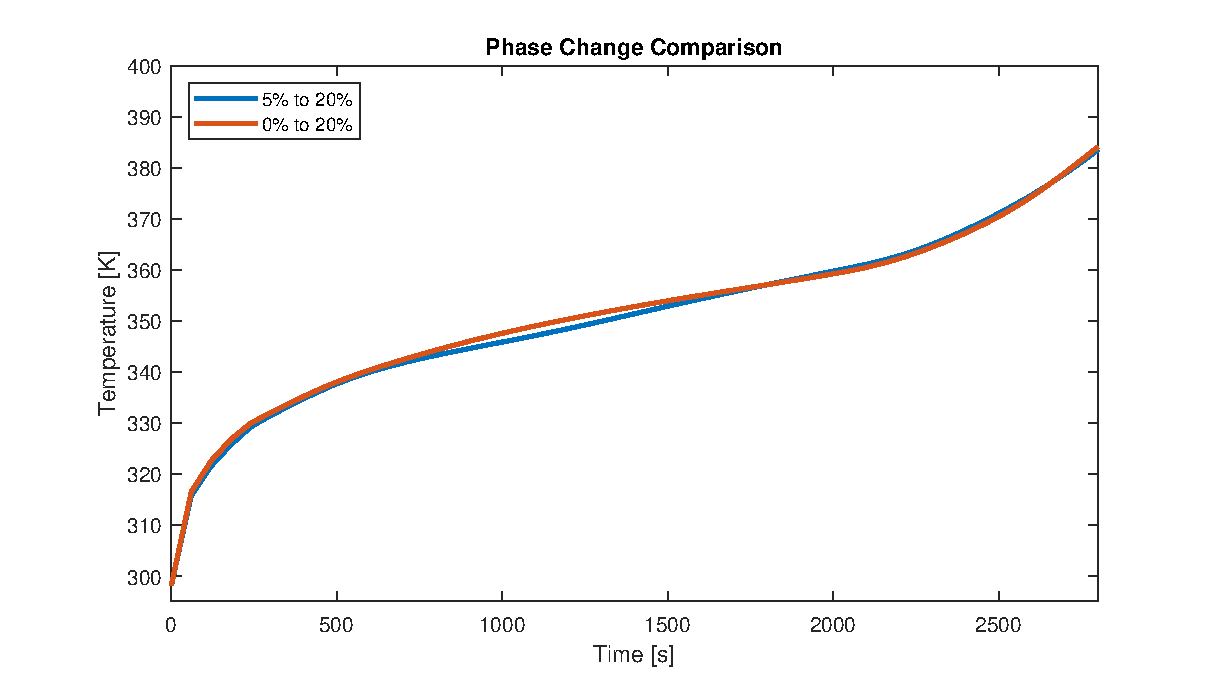
\includegraphics[width=\linewidth]{figures/chapter_4/PhaseChangeComparisonLattice.eps}
    \caption{Temperature evolution over phase change simulation}
    \label{fig:phase_change_lattice}
  \end{subfigure}
  \caption{Topology optimization results obtained using a larger porosity range (left) and the resulting phase change simulation compared to the optimal porosity range (right)}
\end{figure}
  
Another note for these structures is that the range in thermal conductivity is quite small, even when the porosity is 0\%. This is because the phase change material has a fairly high thermal conductivity compared to the maximum. This provides only a small change in the order of magnitude which is why there are minimal branches generated. To determine whether using the lattice material properties provides any benefit, a final structure has been generated that uses generic thermal conductivity in the range of zero to one. The resulting structure, shown in figure \ref{fig:thermal_opt_generic}, has many small branches as well as a lot of gray elements. As has been mentioned, these gray elements are undesirable due to the non-linear nature of the latent heat curve shown in figure \ref{fig:thermal_properties}. As a result, this structure has the lowest total latent heat.
\begin{figure}[ht]
  \centering
  \begin{subfigure}{0.45\linewidth}
    \includegraphics[width=\linewidth]{figures/chapter_4/ThermalOptGeneric.png}
    \caption{Typical thermal topology optimization using generic material properties}
    \label{fig:thermal_opt_generic}
  \end{subfigure}
  \hfill
  \begin{subfigure}{0.5\linewidth}
    \includegraphics[width=\linewidth]{figures/chapter_4/PhaseChangeComparisonLatticeGeneric.eps}
    \caption{Temperature evolution of all the optimized structures}
    \label{fig:phase_change_lattice_generic}
  \end{subfigure}
  \caption{Topology optimization results obtained using generic material properties (left) and the resulting phase change simulation compared to all other structures (right)}
\end{figure}
  
Comparing all the structures in a phase change simulation shows that the lattice properties have a significant benefit in minimizing the temperature. However, this is most likely because the total latent heat available to each system varies. Figure \ref{fig:phase_change_lattice_generic} shows that the structure generated with generic properties performs the worst right from the start. At this point, the system is conduction dominant, so it could imply that the generic properties do not capture the true conductivity well enough to optimize the system. This means that the poor placement of high porosity elements around the heat source prevents the initial heat flux from being diffused quickly through the structure. 

\begin{table}[ht]
  \centering
  \begin{tabular}{c | c | c | c}
    Structure & 5\% - 20\% Porosity & 0\% - 20\% Porosity & Generic properties \\ \hline
    Total Latent Heat [MJ] & 740.207 & 738.489 & 734.139 
  \end{tabular}
  \caption{Total available latent heat in each structure}
  \label{table:latent_heat_available}
\end{table}

To further show that the structure generated for the porosity range of 5\% to 20\% is the best option, another plot has been generated to show the phase fraction of the central node on the heat flux boundary. The plot includes the phase fraction obtained for another structure that was generated for the porosity range of 10\% to 20\%. At the time this node is melting, most of the domain is below the melting temperature, so the domain can be considered as conduction dominant. This is likely why the 5\% to 20\% structure performs the best.
\begin{figure}[ht]
  \centering
  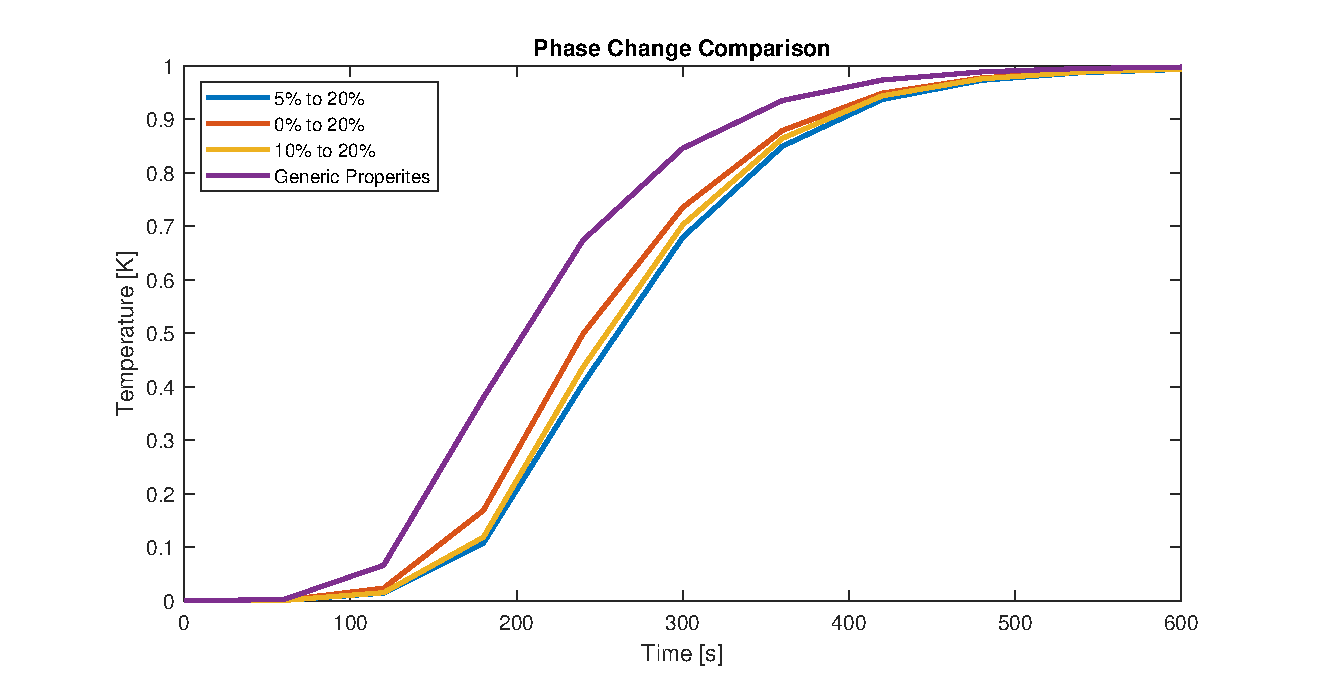
\includegraphics[width=0.7\linewidth]{figures/chapter_4/PhaseFractionRate.eps}
  \caption{Phase fraction at the hottest node in domain}
  \label{fig:phase_fraction}
\end{figure}


\subsection*{Minimising Phase Change Compliance}
This approach appears to be a novel idea where the transient effects are taken into account when finding an optimum. This would be similar to a non-linear topology optimization. The problem with this method is that there is no simple way to compute the derivative of the compliance. Recall that the compliance is defined as shown in equation \ref{eq:thermal_compliance}. However, in the transient phase change problem, the derivation of the element sensitivities can not be used. Beginning with the gradient of the compliance, shown in equation \ref{eq:compliance_gradient_pc}, a new derivation can be achieved which is given in Appendix B.
\begin{equation}
  \frac{\partial c}{\partial \rho} = \frac{\partial\mathbf{T}^T}{\partial\rho}\mathbf{f}+\mathbf{T}^T\frac{\partial\mathbf{f}}{\partial\rho}
  \label{eq:compliance_gradient_pc}
\end{equation}

The main problem with this equation is the $\frac{\partial\mathbf{T}}{\partial\rho}$ which can not be easily computed. Automatic differentiation could be used, but using the \emph{ForwardDiff} library is far too slow to be viable. The main issue is that in the forward pass, each dual variable is traced through the entire program, but most of them have no effect on the final result as the forcing vector $\mathbf{f}$ is mostly zeros. Reverse mode AD could be used instead, but because multiple Newton iterations are needed to resolve the non-linearity very high amounts of memory are required. It is for these reasons the gradient was derived, and has been computed manually.

\subsubsection*{\emph{Implementation}}
The latent heat vector and latent heat matrix can not be computed using automatic differentiation because they require the gradient of the temperature vector w.r.t the relative density. To compute them using AD would mean the entire simulation needs to be computed using AD which is what is being avoided. Here the element's relative density will be denoted using $\varphi$ to avoid confusion with the material density $\rho$. Recall that $N$ is the element shape functions, $L$ is the latent heat, and $f_{pc}$ is the phase fraction. Equation \ref{eq:latent_heat_element_gradient} shows the gradient of the element latent heat vector, and a similar gradient can be obtained for the latent heat matrix.
\begin{equation}
  \begin{split}
    L_e &= \int_{\Omega^e} N \rho(\varphi) L(\varphi)f_{pc}(\varphi)\ d\Omega^e \\
    \frac{\partial L_e}{\partial\varphi} &= \int_{\Omega^e} N \frac{\partial}{\partial\rho_e}\left(\rho(\varphi) L(\varphi)f_{pc}(T)\right)\ d\Omega^e \\
    &= \int_{\Omega^e} N \left( Lf_{pc}\frac{\partial\rho}{\partial\varphi} + \rho f_{pc}\frac{\partial L}{\partial\varphi} + \rho L\frac{\partial f_{pc}(T)}{\partial\varphi} \right) \ d\Omega^e \\
    &= \int_{\Omega^e} N \left( Lf_{pc}\frac{\partial\rho}{\partial\varphi} + \rho f_{pc}\frac{\partial L}{\partial\varphi} + \rho L\frac{\partial f_{pc}(T)}{\partial T}\frac{\partial T}{\partial\varphi} \right) \ d\Omega^e
  \end{split}
  \label{eq:latent_heat_element_gradient}
\end{equation}

Some specific implementation stages have been used in this optimization problem to obtain results as quickly as possible. Because the global matrices are assembled as a sum of the element matrices, the derivative of the matrices w.r.t any element's relative density is simply the derivative of the element matrix. This is illustrated in equation \ref{eq:phase_change_element_derivative}. These element derivatives can be efficiently computed using \emph{ForwardDiff} while computing each finite element matrix.
\begin{subequations}
  \begin{equation}
    \frac{\partial\mathbf{K}}{\partial\rho_e} = \frac{\partial\mathbf{K_e}}{\partial\rho_e}
  \end{equation}
  \begin{equation}
    \frac{\partial\mathbf{C}}{\partial\rho_e} = \frac{\partial\mathbf{C_e}}{\partial\rho_e}
  \end{equation}
  \label{eq:phase_change_element_derivative}
\end{subequations}

\subsubsection*{\emph{Observations}}
The results obtained for the phase change compliance are quite interesting because the results depend on how long the simulation runs. Three example cases have been generated. The first case runs for a longer time than required to have the domain fully melt. This essentially means the gradient is conduction-dominant. The second case only runs for as long as it takes to fully melt the domain. The third case elapses for a fixed time that does not allow the domain to fully melt.

For these structures, a coarse mesh needed to be used to produce results in a reasonable time. Even though the gradients are computed much faster, they still take at least a couple of hours to fully produce. As a result of using a coarser mesh, the filter radius had to be increased. For that reason, the results will be compared to a new pure conduction optimized structure shown in figure \ref{fig:pure_conduction_comparison}.
\begin{figure}[ht]
  \centering
  \includegraphics[width=0.8\linewidth]{figures/chapter_4/PhaseChangeCoparison.png}
  \caption{Pure conduction optimized structure}
  \label{fig:pure_conduction_comparison}
\end{figure}

The first example, which will be referred to as the conduction dominant case, is shown in figure \ref{fig:conduction_dominant_structure}. The produced structure is similar, though much softer than the pure conduction case. Very faint \emph{'ears'} are forming, similar to those that formed in the pure conduction case.
\begin{figure}[ht]
  \centering
  \includegraphics[width=0.8\linewidth]{figures/chapter_4/PhaseChangeConductionDominant.png}
  \caption{Conduction dominant structure}
  \label{fig:conduction_dominant_structure}
\end{figure}

The second example, which will be referred to as the latent heat dominant case, is shown in figure \ref{fig:latent_heat_dominant_structure}. The produced structure is much different from the previous two. In this case, the latent heat effects don't have time to be overpowered by the conduction effects. This structure contains two strong branches, which should in theory sustain a larger melting front. This means that the temperature should be held constant for a longer time.
\begin{figure}[ht]
  \centering
  \includegraphics[width=0.8\linewidth]{figures/chapter_4/PhaseChangeLatentHeatDominant.png}
  \caption{Latent heat dominant structure}
  \label{fig:latent_heat_dominant_structure}
\end{figure}

The third example, which will be referred to as the incomplete melting case, is shown in figure \ref{fig:incomplete_melting_structure}. This structure was optimized for the end time of 1800 seconds, or 30 minutes. This structure is very similar to the conduction dominant structure, except it has a larger \emph{"smoothing"} radius. This likely means the melting front is smoother, which should subject more elements to melting at once. What is obviously expected is that this structure should perform the best for the time that it was fixed, but will likely perform worse overall.
\begin{figure}[ht]
  \centering
  \includegraphics[width=0.8\linewidth]{figures/chapter_4/PhaseChangeIncompleteMelting.png}
  \caption{Incomplete melting structure}
  \label{fig:incomplete_melting_structure}
\end{figure}

To be able to compare all the structures that have been obtained, a phase change simulation has been performed for each. Figure \ref{fig:phase_change_optimal_comparison} shows the maximum temperature over time for each structure. The results are similar for each, but what is most interesting is that the pure conduction case performs the worst. The total latent heat available to that structure was the greatest of each of the examples. This highlights the fact that total latent heat does not ensure the best possible structure, but rather the placement of the \emph{grey} elements is more important. It also shows that optimizing for phase change can provide a benefit. 
\begin{figure}[ht]
  \centering
  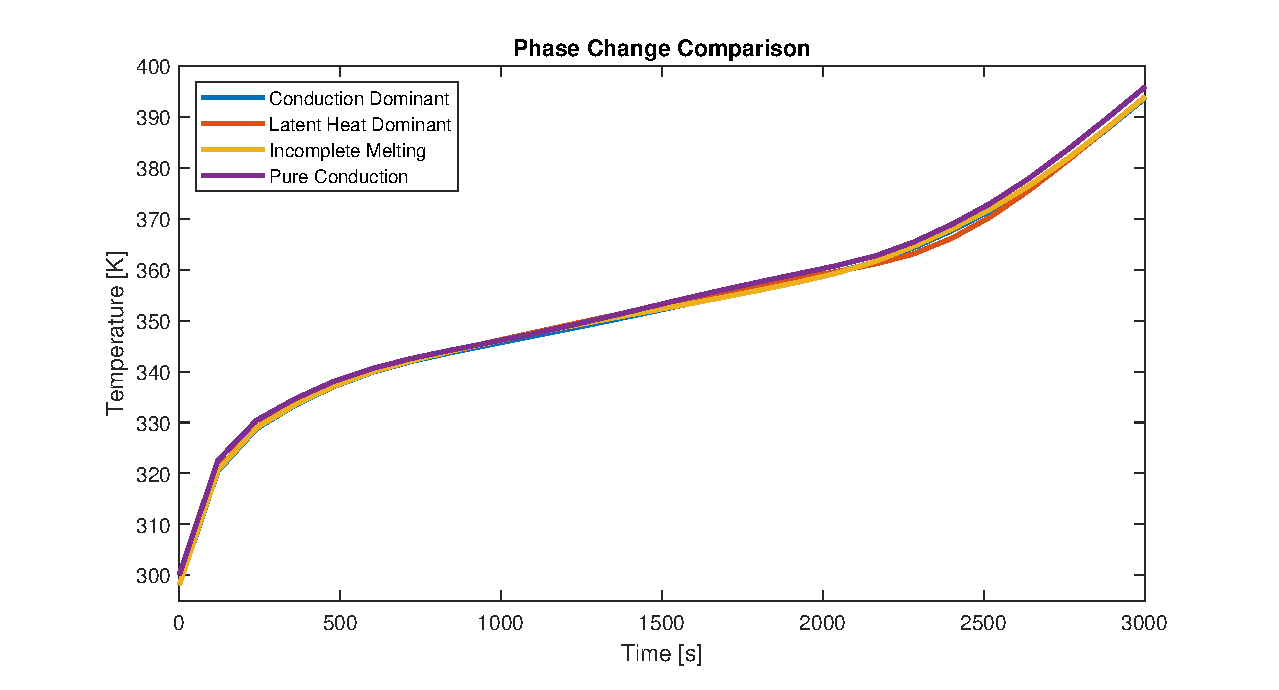
\includegraphics[width=0.8\linewidth]{figures/chapter_4/PhaseChangePhaseChangeComparison.eps}
  \caption{Phase change simulation results}
  \label{fig:phase_change_optimal_comparison}
\end{figure}

The differences between the phase change optimal structures, on the other hand, are almost insignificant. What is most interesting, however, is that the incomplete melting case does perform best until the time it was optimized for. This is to be expected but highlights an important consideration that needs to be made if the structure is not expected to fully melt.

What is not very clear from the plot is that the latent heat dominant example does keep the temperature lower for longer, but after enough time has elapsed, the temperature rises to the same as the conduction dominant case. This result is also important, because if the goal is to keep the temperature constant for as long as possible, then a latent-heat-optimized structure should be generated. In this example, it was kept cooler for around 200 seconds longer, which could provide some benefit to some systems.

The time cost of producing the phase change optimized structures is quite significant. Many aspects of the code could be optimized and parallel computing could be implemented, but even so, for 3D structures with a fine mesh, the time to produce a structure could take many hours and would likely exceed a day.


\section{Remarks}
From the results obtained for the single functional components of this thesis, it is already clear that using lattice properties plays an important role in the kinds of structures that are produced. One can not simply neglect the lattice properties and use generic properties, as could be done for traditional topology optimization. This is because the \emph{empty} regions with a relative density of $0$ still provide a significant amount of stiffness or conduction which helps to minimize the compliance.

Based on results from both the refinement studies that were conducted, a trade-off between mesh size and filter radius needs to be reached. Using a coarse mesh produces the same structure as the finest mesh, but results in a large filter radius being required. This reduces the performance of the structure, especially in the structural problem. Using the finest mesh, however, increases the computational cost. Furthermore, high-resolution structures are produced that can not be realized in the lattice structure after homogenization. 

It is also clear that optimizing for phase change can provide some benefits. However, this benefit comes at a high computational cost that could severely limit its usability to general uses. In the future, more work needs to be done to simplify, accelerate and optimize the performance of this module to make it scalable to 3D domains.